\chapter[Resultados]{Resultados}

Baseando-se nos métodos e materiais descritos no capítulo \ref{chap:materials-and-methods}, iniciou-se a etapa de desenvolvimento e organização dos dados a partir da \textit{pipeline} de \textit{crappier} para a imagens, para então testar a hipótese do projeto. O presente capítulo mostra, de maneira detalhada, o que foi feito para realizar o levantamento e criação dos dados de imagens necessárias para serem consumidas pelos pré-processadores de imagem que visam melhorar a qualidade do OCR extraído dos textos, bem como a comparação dos mesmos por meio das métricas propostas.

\section{Infraestrutura}

Para o desenvolvimento do projeto foi utilizado um Sistema Operacional  Pop!\_OS 20.04 LTS baseado em GNU/Linux, com 16GB de memória RAM, disco com capacidade de 1.2 Terabytes de armazenamento, processador AMD® Ryzen 5 3600 com 6 (seis) \textit{cores} e 12 (doze) \textit{threads} e uma placa de vídeo dedicada NVIDIA GeForce RTX 2060 com 6GB de capacidade. Para os processamentos em placa gráfica foram utilizados o CUDA na versão 11.1 e o CuDNN na versão 10.


\section{Tratamento e formação do \textit{dataset}}

\subsection{Separação de documentos}
O conjunto de PDFs fornecidos como dados estavam todos juntos em um único diretório no disco, sem a correta divisão de qual era o dado contido no PDF. O CSV fornecido pelo GPAN e os itens descritos na tabela \ref{tab:csv-details} fazem referência a todas as páginas desses PDFs e possui também o seu conteúdo, sendo eles extraídos por meio de OCR ou não, como mostra a figura \ref{fig:gpan-pipeline}. Porém como o foco do trabalho é realizar estudos sobre a qualidade do OCR, decidiu-se por separar o dado entre os que foram extraídos utilizando OCR dos que não foram.

Para isso, gerou-se um novo CSV apenas com os registros de páginas cujo necessitou-se do OCR em sua extração e criou-se também um diretório para armazenar apenas os PDFs que possuíam páginas não-selecionáveis. Dos 89.578 arquivos, existem cerca de 354.501 páginas somadas, sendo essas:

\begin{table}[H]
  \centering
  \caption{Divisão de páginas dos PDFs.}
  \begin{tabular}{|m{10em}|c|}
    \hline
      \textbf{Tipo}  &
      \textbf{Quantidade} \\
    \hline
      Necessita de OCR  &
      80.624 \\
    \hline
      Não necessita de OCR  &
      273.877 \\
    \hline
      \textbf{TOTAL}  &
      \textbf{354.501} \\
    \hline
  \end{tabular}
  \legend{Fonte: autoral}
  \label{tab:csv-diff}
\end{table}

\subsection{Extração de imagem do PDF}
Com os dados separados em um diretório específico, iniciou-se a etapa de extração de imagem a partir dos documentos em formato PDF dos processos. Utilizou-se também informações do CSV (tabela \ref{tab:csv-details}) para selecionar a página específica do documento a qual o OCR foi utilizado, diminuindo assim o tempo de processamento por documento.

A extração de imagem a partir do PDF é feita utilizando um algoritmo de software livre desenvolvido em Python, chamado de \textit{pdf2image}. Ele recebe como entrada um PDF e é possível definir qual ou quais páginas do PDF deseja-se extrair, permitindo assim a geração do \textit{dataset} de imagens de processos.

\subsection{Aplicação de filtros}
Para a criação de um modelo generativo que consiga diminuir os ruídos de imagens, é preciso utilizar como dado de entrada imagens que possuam tais características - ruídos. Das 354 mil páginas dos PDFs disponíveis, fazer a separação de todas elas para a identificação de imagens ruins deria um trabalho bem complexo e que diminuiria o tempo disponível para o desenvolvimento do presente trabalho. Com isso, adotou-se a heurística de que todas as fotos que tiveram texto extraído via OCR (tabela \ref{tab:csv-diff}) seriam "pioradas" \  aplicando um conjunto de filtro de imagens de diferentes tipos.

Um filtro de imagem é um algoritmo ou rotina de software que consegue alterar de forma fixa ou aleatória os valores dos pixels contidos em uma imagem. Com isso, é possível criar uma lógica que tente simular imagens escaneadas de maneira automatizada, aplicando sombreamento, borrões, manchas, distorções, etc.


\begin{figure}[H]
  \centering
  \caption{Diferença entre uma foto original e uma com filtro}
  \begin{subfigure}{.5\textwidth}
    \centering
    \caption{Foto sem filtro}
    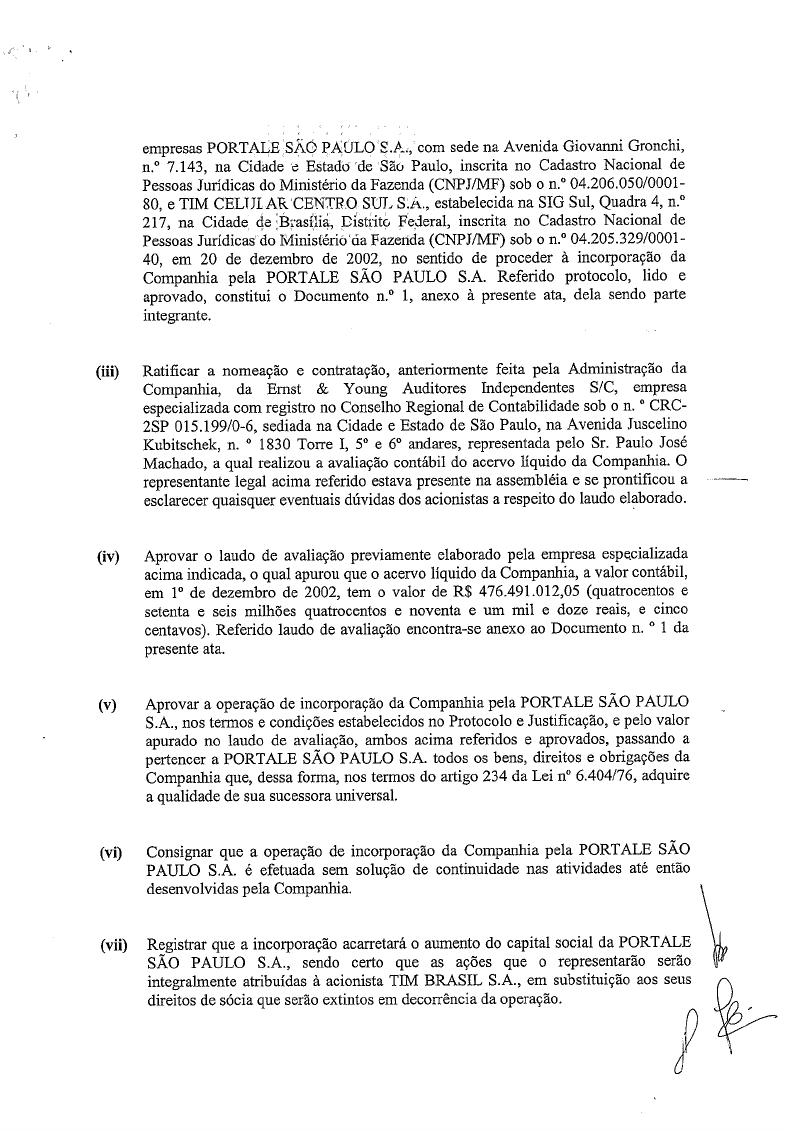
\includegraphics[width=0.8\linewidth]{figuras/good-text-image.jpg}
    \label{fig:image-without-filter}
  \end{subfigure}%
  \begin{subfigure}{.5\textwidth}
    \centering
    \caption{Foto com filtro aplicado}
    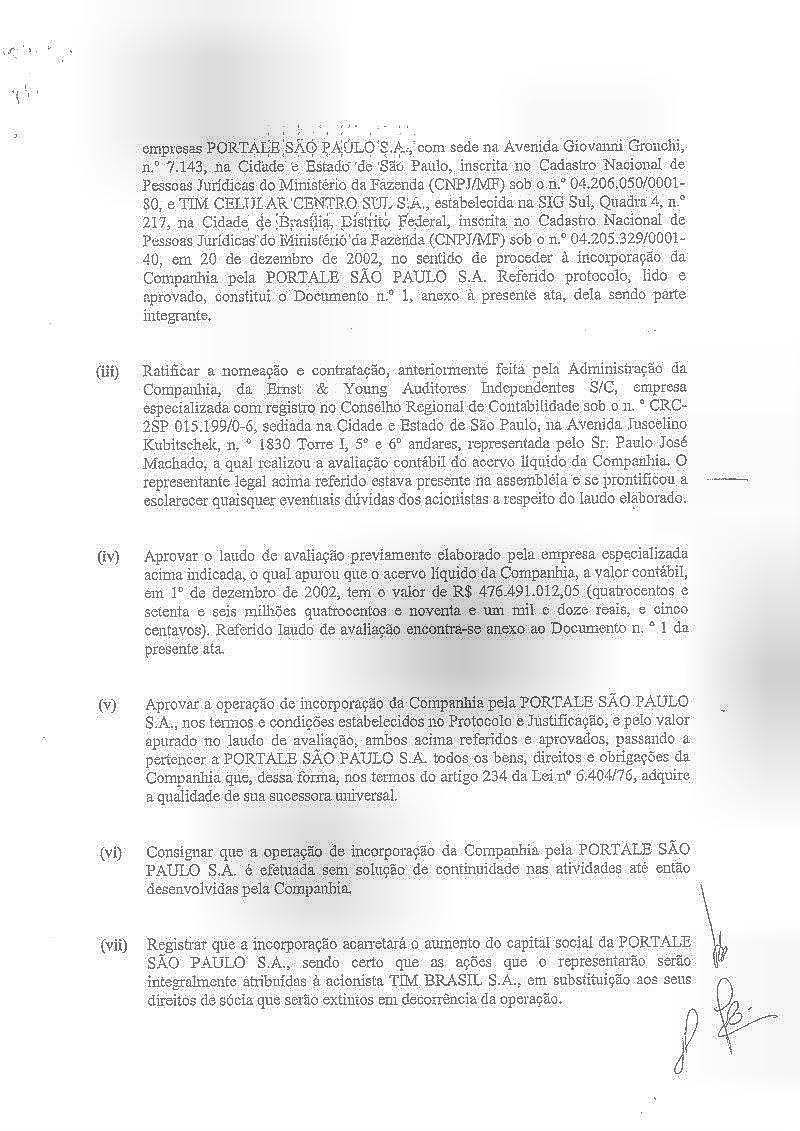
\includegraphics[width=0.8\linewidth]{figuras/image-with-overlay.jpg}
    \label{fig:image-with-filter}
  \end{subfigure}
  \legend{Fonte: autoral}
  \label{fig:side-process-images}
\end{figure}

Existem diversas bibliotecas já implementadas em Python que possibilitam a aplicação de filtros em imagens. As utilizadas foram: \textit{ImageFilter} da biblioteca \textit{Python Imaging Library} e \textit{imgaug}, biblioteca de \textit{data augmentation}\footnote{
  Processo de transformação do dado que permite que seu volume ou amostra cresça, fornecendo assim mais insumos ou entradas de dados disponíveis em um processo de treinamento de algoritmo.
}. Alguns filtros foram de origem autoral.

Abaixo, listam-se todos os filtros utilizados e estudados para o presente processamento de imagem.

\begin{table}[H]
  \centering
  \caption{Descrição dos filtros utilizadosverbo tesselar.}
  \begin{tabular}{|m{.25\linewidth}|m{.1\linewidth}|m{.55\linewidth}|}
    \hline
      \textbf{Nome}  &
      \textbf{Fonte}  &
      \textbf{Descrição} \\
    \hline
      EDGE\_ENHANCE  &
      PIL  &
      Aumenta o contraste dos píxels ao redor de bordas para que essas bordas se destaquem mais do que os demais elementos da foto  \\
    \hline
      CONTOUR  &
      PIL  &
      Similar ao EDGE\_ENHANCE mas com maior intensidade \\
    \hline
      RandomOverlay  &
      autoral  &
      Cria formas gerométricas randômicas e transparentes e as coloca acima da imagem original, dando a impressão de manchas. A posição das formas também é randômica. \\
    \hline
      PerspectiveTransform  &
      \textit{imgaug}  &
      Aplica randomicamente transformações de 4 pontos de perspectiva, dando uma ideia de "lupa" para algus pontos da imagem \\
    \hline
      SaltAndPepper  &
      \textit{imgaug}  &
      Substitui píxels randômicos da imagem por píxel de sal (cor branca) e pimenta (cor preta) \\
    \hline
      GammaContrast  &
      \textit{imgaug}  &
      Ajusta o contraste da imagem escalando os píxels da imagem em um valor calculado por \(x = 255(\frac{v}{255})^{\gamma}\), onde $\gamma$ é um parâmetro da função entre $0$ a $1$ e $v$ é o antigo valor do píxel \\
    \hline
      JpegCompression  &
      \textit{imgaug}  &
      Degrada a imagem aplicando uma compressão de JPEG, diminuindo sua qualidade \\
    \hline
      Dropout  &
      \textit{imgaug}  &
      Randomicamente coloca uma fração de pixels da imagem para o valor 0 \\
    \hline
      Affine  &
      \textit{imgaug}  &
      Aplica transformações na imagem mas mantém relações de colinearidade e distância. Geralmente composta por rotações, translações e dilatações das formas presentes na imagem. \\
    \hline
  \end{tabular}
  \legend{Fonte: autoral}
  \label{tab:sdas}
\end{table}

As tecnologias de OCR disponíveis, como o Tesseract, em geral são muito sensíveis e aplicar todos esses filtros em uma única imagem impede que o OCR identifique caracteres nas mesmas. Com isso, é preciso escolher randomicamente entre os filtro listados, podendo aplicar um ou mais deles, mas nunca podendo aplicar todos de uma só vez.

O processo seguido para a criação de imagens ruins foi de que, para cada uma imagem boa, gera-se uma imagem ruim. Isso se dá pela alta quantidade de imagens disponíveis para treinamento, visto que se for necessário o consumo de mais imagens para treinamento na etapa de geração do modelo, é possível utilizar de \textit{data augmentation} para ampliar a base de dados.

\begin{figure}[H]
  \centering
  \caption{Geração de imagens atual vs geração com \textit{data augmentation}}
  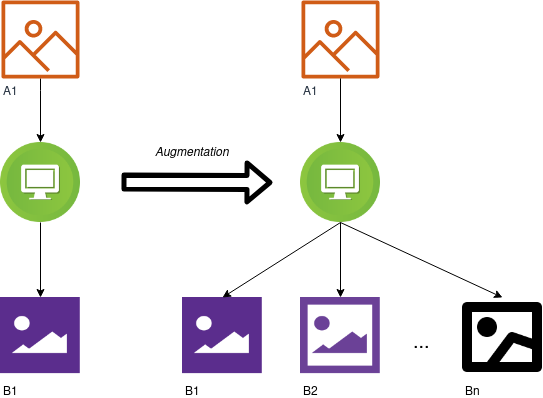
\includegraphics[scale=.6]{figuras/data-augmentation.png}
  \legend{Fonte: autoral}
  \label{fig:data-augmentation}
\end{figure}

\subsection{Extração de texto via OCR}

Para a extração de caracteres utilizando o OCR, fez-se o uso da tecnologia Tesseract, que atualmente consegue identificar e reconhecer mais de 100 idiomas por meio da configuração \textit{unicode}\footnote{
  Padrão que permite que os sistemas informatizados representem e manipulem textos de quaisquer idiomas de escrita que existem na atualidade. Fonte: Wikipedia.
}. Para tal, configura-se o Tesseract com a extensão para a lingua portuguesa, já disponível pela comunidade para uso.

Todo o texto extraído é armazenado em um CSV de saída que identifica qual o processo, documento e página que a extração foi feita. Isso depois servirá como base para a verificação e métrica para a comparação entre o texto extraído de uma página limpa para uma página com ruídos.

O texto extraído das imagens ruins foram comparados previamente para verificar se o OCR estava realmente pior do que o texto original, a partir da métrica ROUGE-1. A seguir, mostra-se um exemplo de imagens e suaas respectivas extrações de texto utilizando OCR, sendo a primeira da imagem original e a segunda da imagem \textit{crappy}, respectivamente.

\begin{figure}[H]
  \centering
  \caption{Imagem de boa qualidade}
  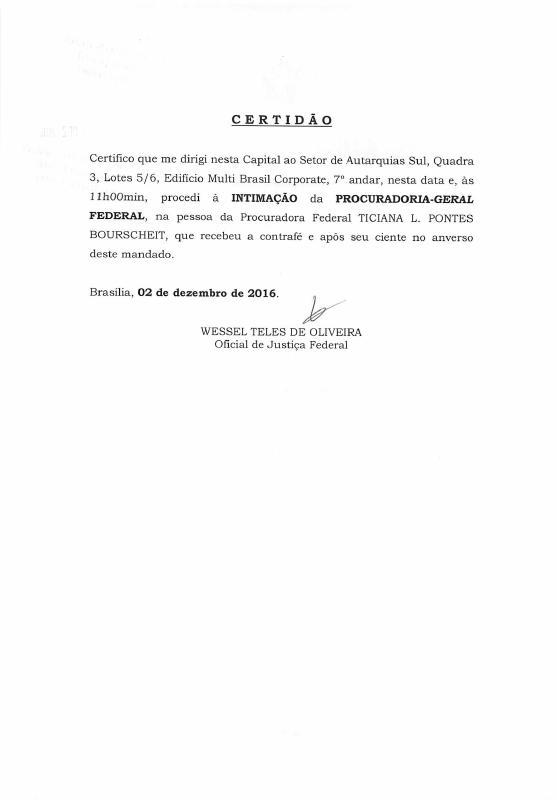
\includegraphics[scale=.6]{figuras/good-image-extracted.jpg}
  \legend{Fonte: STF.}
  \label{fig:good-image-extracted}
\end{figure}

\begin{alltt}
          CERTIDÃO

          Certifico que me dirigi nesta Capital ao Setor de
          Autarquias Sul, Quadra 3, Lotes 5/6, Edificio Multi
          Brasil Corporate, 7º andar, nesta data e, às
          11h00min, procedi à INTIMAÇÃO da PROCURADORIA-GERAL
          FEDERAL, na pessos da Procuradora Federal TICIANA L. PONTES
          BOURSCHEIT, que recebeu a contrafé e após seu
          ciente no anverso deste mandado.

          Brasília, 02 de dezembro de 2016,

          WESSEL TELES DE OLIVEIRA
          Oficial de Justiça Federal
\end{alltt}

\begin{figure}[H]
  \centering
  \caption{Imagem gerada pelo \textit{crappier} \textit{pipeline}}
  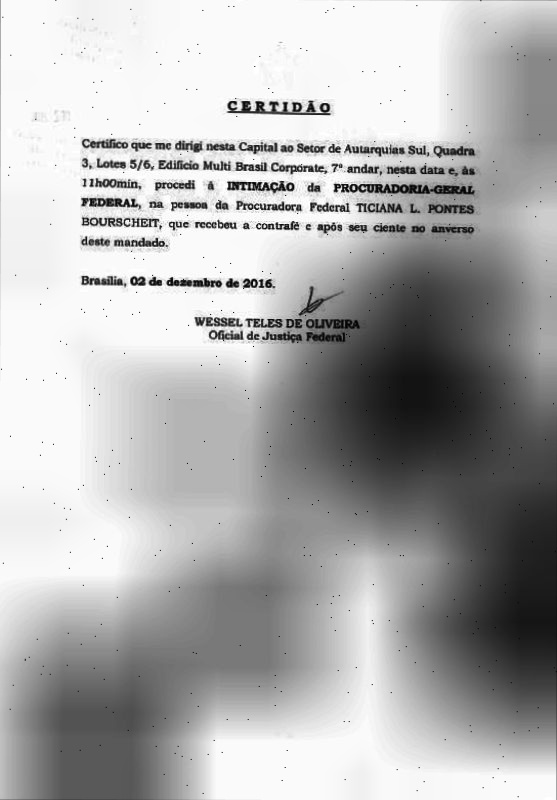
\includegraphics[scale=.6]{figuras/bad-image-extracted.jpg}
  \legend{Fonte: autoral.}
  \label{fig:bad-image-extracted}
\end{figure}

\begin{alltt}
          CERTIDÃO

          Certífico que me dirigi nesta Capital ao Setor de
          Autarquias Sul, Quadra. 4 , Lotes 5/6, Edifício Muki
          Brasil Corpórate, 7º andar, nesta
          11h00Min, procedi à INTIMAÇÃO da
          FEDERAL, na pesson da Procuradora Federal TICIANA
          BOURSCHEIT, que recebeu a contrafé e apõs sem
          deste mandado.

          Brasília, 02 de desembro de 2016.
\end{alltt}

Foi possível então verificar, assim como no exemplo acima, que a qualidade de extração do OCR piorou em comparação com o texto original. Neste exemplo, ao ser aplicada a métrica ROUGE-1, obteve-se como \textit{score} o valor de $0.65$, mostrando que existem diferenças significativas dentro do texto.

Permite-se então validar que o \textit{dataset} gerado poderá servir de insumo para as etapas futuras do desenvolvimento do projeto.

\section{Pré-processadores de Imagem}

Com todo o \textit{dataset} devidamente construído, é possível prosseguir com a construção dos pré-processadores de imagens. Para validar os estudos propostos, criou-se 3 (três) tipos diferentes de processadores:

\begin{itemize}
  \item Processador de Imagem simples;
  \item Processador GAN;
  \item Processador \textit{Decrappification};
\end{itemize}

\begin{figure}[H]
  \centering
  \caption{Processo de correção de imagem, extração de texto e criação de métricas}
  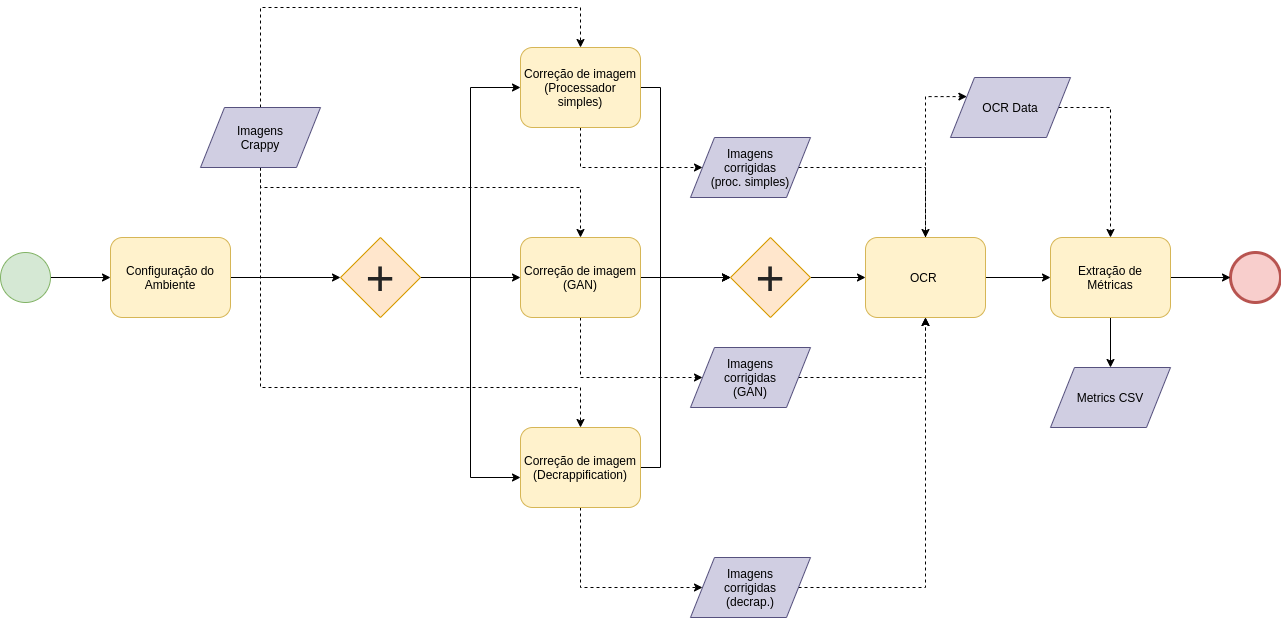
\includegraphics[scale=.5, angle=270]{figuras/text-extraction-and-comparison-flow.png}
  \legend{Fonte: autoral.}
  \label{fig:text-extraction-and-comparison-flow}
\end{figure}

O processo de construção dos mesmos, bem como exemplos de seus resultados serão apresentados a seguir.

\subsection{Pocessador de Imagem simples}

Com os dados já estruturados e o processo de validação da hipótese desenhado, iniciou-se a construção do primeiro pré-processador de imagem, que consiste em utilizar mecanismos de processamento de imagem convencionais com o propósito de tratar a imagem de entrada do OCR a fim de atingir melhores resultados.

Tal pré-processador possui 4 (quatro) etapas em sua construção, assim como foi listado na seção \ref{sec:filtro-de-imagem}, mas com a adição de correção de expessura das linhas da imagem \cite{K3M-image-skeletonization}. Cada uma delas será discutida a seguir.

O pré-processador foi construído baseado na biblioteca OpenCV para Python em sua versão 4.4.

\subsubsection{Binarização} \label{sssec:binarization}

Como citado na seção \ref{sec:filtro-de-imagem}, a binarização consiste em converter os pixels da imagem entre 0 ou 255 - uma analogia entre o 0 e 1 da nomenclatura binária - a partir de um valor de referência, ou \textit{threshold}. Porém, quando lida-se com imagens e ruídos não conhecidos, é importante considerar que nem todo pixel corrigido no processo de binarização será alterado para o valor correto.

\begin{figure}[H]
  \centering
  \caption{Binarização simples considerando \textit{threshold} = 127}
  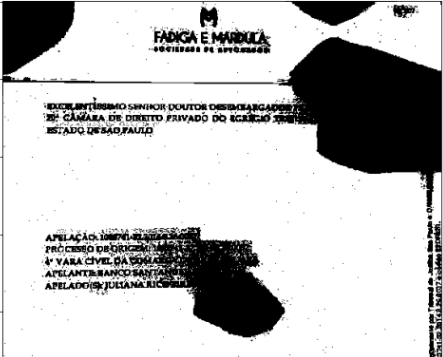
\includegraphics[scale=.7]{figuras/binarizacao-simples.png}
  \legend{Fonte: autoral.}
  \label{fig:binarizacao-simples}
\end{figure}

A biblioteca do OpenCV implementa, até o desenvolvimento do presente trabalho, 5 (cinco) funções de binarização diferentes no mesmo algoritmo, definido por parametrização da função de \textit{threshold}. Para verificar qual desses parâmetros apresentariam melhores resultados, utilizou-se a métrica de \textit{Mean Square Error} \cite{mse-metric}, métrica utilizada para medir a qualidade da imagem baseada na imagem referência que será explicada em mais detalhes na seção \ref{ssec:processor-gan}. Utilizando um  \textit{sample} dos dados originais junto aos dados \textit{crappy}, foi possível verificar quais desses valores melhor se adequam ao dado. Na métrica MSE, quanto menor o valor resultante, melhor é a qualidade da imagem \cite{mse-metric} resultante.

\begin{figure}[H]
  \centering
  \caption{métrica MSE para a comparação dos diferentes valores de binarização simples}
  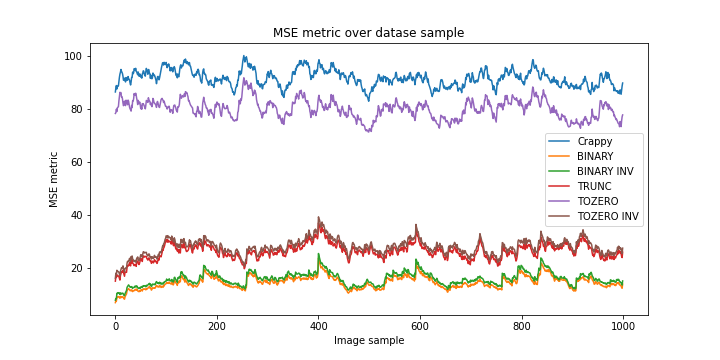
\includegraphics[scale=.63]{figuras/smoothed-binarization-test.png}
  \legend{Fonte: autoral.}
  \label{fig:smoothed-binarization-test}
\end{figure}

Apenas observando a métrica, é possível verificar que os valores de \textit{BINARY} e \textit{BINARY INV} são os que apresentaram os menores valores. Porém, como mostrado na figura \ref{fig:binarizacao-simples}, os algoritmos de binarização simples não são adequados para o dado em questão, visto que uma binarização absoluta com valores entre 0 e 255 resulta na perda de informação considerável na imagem. Portanto, o algoritmo que obteve o melhor resultado após o descarte dos citados anteriormente foi o \textit{TRUNC}, representado pela seguinte função matemática:

\begin{gather}
  d(x,y) =
  \begin{cases}
    \text{\textit{threshold}}, & \text{se } s(x,y) > \text{\textit{threshold}} \\
    s(x,y), & \text{se não}
  \end{cases}
  \label{math:threshold-trunc}
\end{gather}

Considerando a mesma imagem utilizada para criar a figura \ref{fig:binarizacao-simples} e aplicando-se o filtro com o parâmetro \textit{TRUNC}, tem-se:

\begin{figure}[H]
  \centering
  \caption{Binarização com parâmetro \textit{TRUNC} considerando \textit{threshold} = 127}
  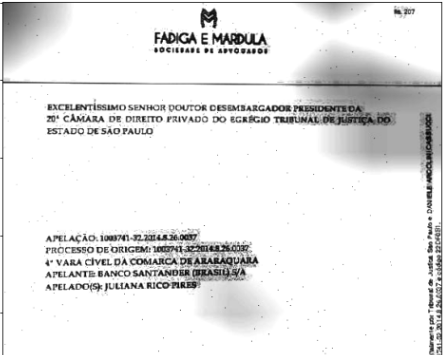
\includegraphics[scale=.7]{figuras/binarizacao-simples-trunc.png}
  \legend{Fonte: autoral.}
  \label{fig:binarizacao-simples-trunc}
\end{figure}

O resultado é uma imagem consideravelmente mais legível e limpa.

Porém, a binarização simples de valores fixos não consegue atingir resultados satisfatórios vindos de superfície de iluminação ou fundo não uniforme \cite{adaptative-threshold-surfaces}. A solução para esse tipo de caso é fazer o uso da binarização adaptativa, que consiste em considerar, além do pixel que está sendo analisado, outros \textit{n} (\textit{kernel} de tamanho \textit{n}) pixels vizinhos do mesmo, calculando o seu valor baseado nos valores ao seu redor \cite{adaptative-threshold-surfaces}. O valor do \textit{threshold} nesse algoritmo pode variar a cada região considerada para a análise. O resultado final da combinação da binarização simples e da binarização adaptativa é mostrado na imagem a seguir.

\begin{figure}[H]
  \centering
  \caption{Binarização adaptativa  em conjunto com binarização simples considerando \textit{threshold} = 127}
  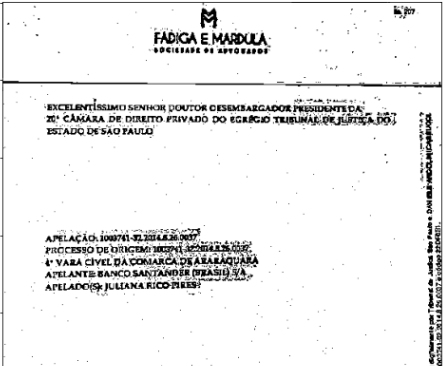
\includegraphics[scale=.7]{figuras/binarizacao-adaptativa.png}
  \legend{Fonte: autoral.}
  \label{fig:binarizacao-adaptativa}
\end{figure}

\subsubsection{Remoção de Ruídos}

O passo seguinte para o pré-processamento de imagem é o de remoção de ruídos. Como citado na seção \ref{ssec:image-denoising}, a remoção de ruídos consiste em conseguir tornar a imagem mais limpa mas mantendo suas principais características. Similar a binarização adaptativa citada em \ref{sssec:binarization}, é possível realizar a redução de ruídos da imagem utilizando o \textit{Non-Local Means Denoising} (NLMD) \cite{non-local-means-denoising}, que também considera uma certa quantidade de pixels ao redor do pixels que está sendo analisado, mas não necessariamente estejam perto do mesmo \cite{non-local-means-denoising}.

A imagem resultante a binarização é a entrada para o algoritmo de remoção de ruídos NLMD, e como resultado tem-se:

\begin{figure}[H]
  \centering
  \caption{Resultado da binarização com redução de ruídos.}
  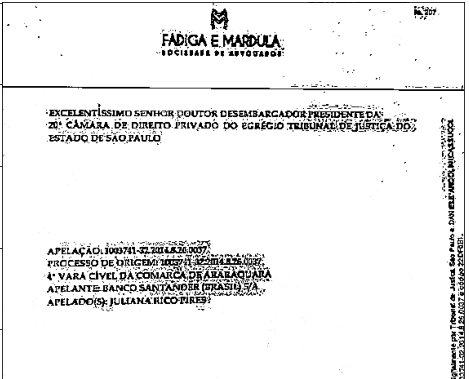
\includegraphics[scale=.7]{figuras/denoising-after-binarization.png}
  \legend{Fonte: autoral.}
  \label{fig:denoising-after-binarization}
\end{figure}

O principal ruído reduzido nesse processo são os resquícios dos ruídos de \textit{Salt And Pepper} vistos na tabela \ref{tab:sdas}. A implementação desse filtro foi possível utilizando a função \href{https://docs.opencv.org/master/d1/d79/group__photo__denoise.html#ga76abf348c234cecd0faf3c42ef3dc715}{\textit{fastNlMeansDenoising}} e os parâmetros foram os valores padrão já configurados da mesma.

\subsubsection{Correção de inclinação}

Além dos ruídos de iluminação não homogênea e manchas na imagem que foram minimizados pelos filtros citados anteriormente, um ponto crucial para a qualidade dos algoritmos de OCR são as questões de alinhamento de texto \cite{ocr-survey} presente na imagem, mostrado na seção \ref{ssec:skew-correction}. De maneira geral, a angulação para a correção do texto é mais evidente quando o mesmo apresenta bastante conteúdo textual na imagem, pois a função que calcula o ângulo possui mais parâmetros para definir o mesmo.

\begin{figure}[H]
  \centering
  \caption{Correção de inclinação da imagem.}
  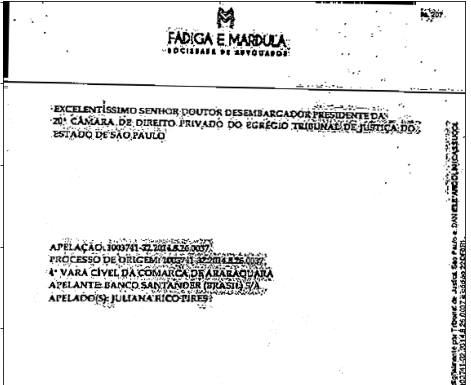
\includegraphics[scale=.7]{figuras/skew-corrected-image.png}
  \legend{Fonte: autoral.}
  \label{fig:skew-corrected-image}
\end{figure}


\subsubsection{Thinning e Skeletonization}

Por último, foi testado também no \textit{dataset} os algoritmos que deixam as linhas presentes na imagem mais espessas ou mais finas, algo similar a "afinar" as curvas, a depender de como os parâmetros são configurados. Porém, o sinal - conteúdo - das imagens de texto do dado estudado em questão representa uma pequena parcela da imagem e transformar linhas das letras não teve efeito positivo, visto que já são pequenas em relação ao restante da imagem.

\subsubsection{Resultados}

Para a validação dos resultados do pré-processador de imagem utilizando filtros de imagem simples separou-se uma amostra aleatória de 1000 (mil) imagens do \textit{dataset} para a comparação entre o OCR resultante das imagens original, \textit{crappy} e corrigida. Durante esse processo, calculou-se também o tempo necessário para limpar a imagem com o pré-processador com a finalidade de comparar, além da qualidade do texto extraído, o tempo médio de limpeza da imagem. A seguir é possível ver a imagem resultante do pré-processador simples implementado.

\begin{figure}[H]
  \centering
  \caption{Exemplo de correção de ruído de imagem.}

  \begin{subfigure}[t]{.3\linewidth}
    
\includegraphics[width=\textwidth]{figuras/991665_310196612_46.jpg}
    \caption{Original}
  \end{subfigure}
  \begin{subfigure}[t]{.3\linewidth}
    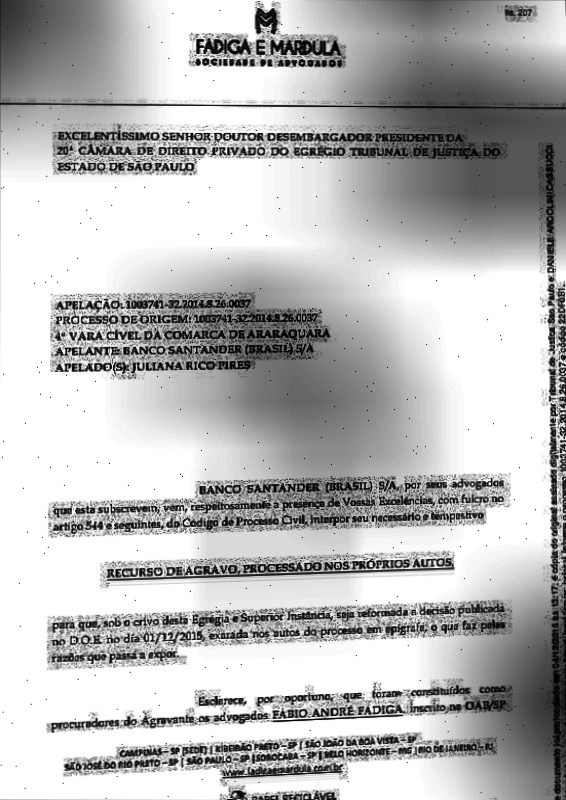
\includegraphics[width=\textwidth]{figuras/991665_310196612_46_crappy.jpg}
    \caption{\textit{Crappy}}
  \end{subfigure}
  \begin{subfigure}[t]{.3\linewidth}
    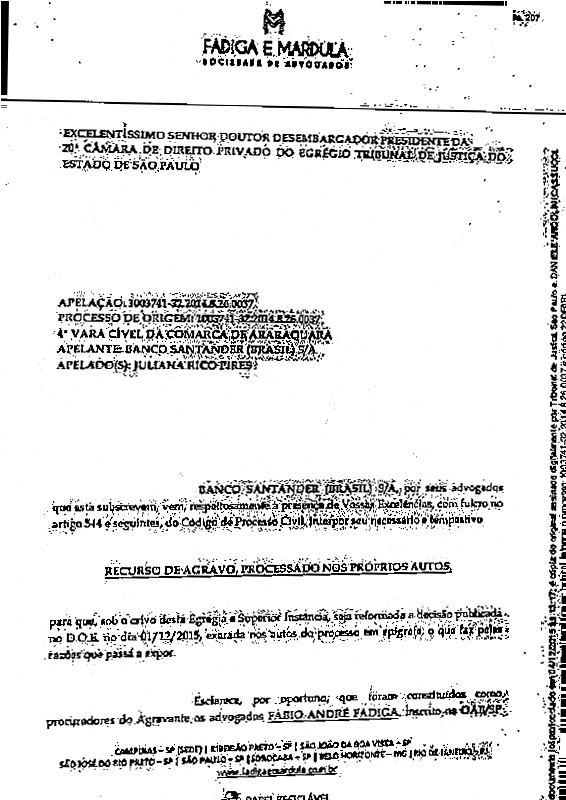
\includegraphics[width=\textwidth]{figuras/991665_310196612_46_corrected.jpg}
    \caption{Corrigida}
  \end{subfigure}
  \legend{Fonte: autoral.}
  \label{fig:skew-corrected-image}
\end{figure}

O resultado final da métrica Rouge-N e Rouge-L, bem como o tempo médio necessário para realizar a "limpeza" da imagem \textit{crappy} pelo pré-processador são vistos nas tabelas a seguir.

\begin{table}[H]
  \centering
  \caption{Tempo médio de processamento da imagem pelo pré-processador simples.}
  \begin{tabular}{|c|}
    \hline
      \textbf{Tempo médio} \\
    \hline
      0.279 segundos \\
    \hline
  \end{tabular}
  \legend{Fonte: autoral}
  \label{tab:pre-processor-average-time}
\end{table}

\begin{table}[H]
  \centering
  \caption{Resumo dos resultados do pré-processador simples.}
  \begin{tabular}{|c|c|c|}
    \hline
      \textbf{Métrica}  &
      \textbf{Crappy}  &
      \textbf{Imagem corrigida} \\
    \hline
      Rouge-1  &
      0.34ms &
      273.877 \\
    \hline
      Rouge-2  &
      0.34ms &
      273.877 \\
    \hline
      Rouge-3  &
      0.34ms &
      273.877 \\
    \hline
      Rouge-4  &
      0.34ms &
      273.877 \\
    \hline
      Rouge-L &
      0.34ms &
      273.877 \\
    \hline
  \end{tabular}
  \legend{Fonte: autoral}
  \label{tab:pre-processor-result}
\end{table}

\subsection{Pocessador GAN} \label{ssec:processor-gan}

Como já citado em momentos anteriores, uma das tecnologias a serem consumidas para o presente trabalho é utilizar um Modelo de DL com foco em minimizar os ruídos das imagens. O primeiro modelo a ser utilizado envolve as GANs \cite{generative-adversarial-networks} para a configuração de um modelo Generativo que receba uma imagem ruim de entrada e gere uma nova, preferencialmente removendo os ruídos da mesma. Com essa proposta, o modelo Generativo tem que necessariamente mapear as principais características de uma imagem para a outra, o que é comumente visto em uma das classes da visão computacional, chamado de \textit{image-to-image translation} \cite{image-to-image-can} ou tradução imagem-para-imagem.

Essa abordagem consiste em aprender as principais características entre as imagens e, dado uma foto de entrada, o modelo consegue adaptar as características da imagem para o formato da sua correspondência. Isso vai desde mapear imagens bidimensionais para imagens de satélite até transformar imagens de uma estação do ano para outra, a partir de uma base de dados suficiente \cite{image-to-image-can}.

\begin{figure}[H]
  \centering
  \caption{Conversão de um mapa 2D para visão aérea ou de satélite.}
  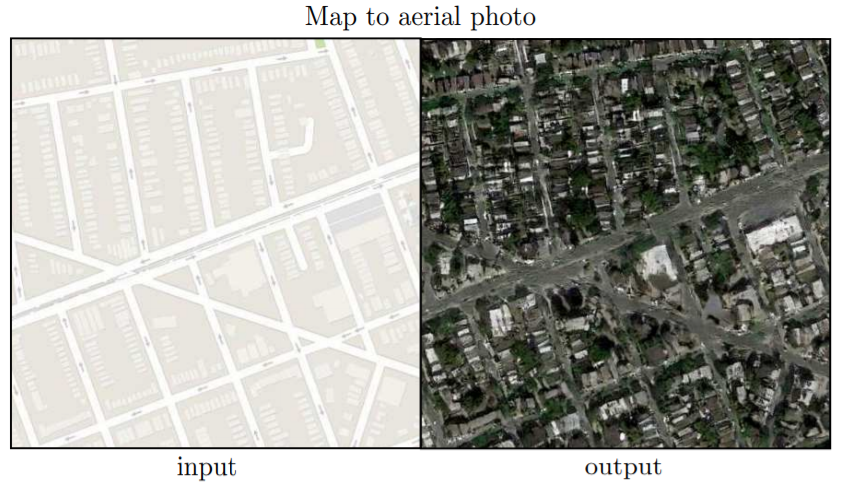
\includegraphics[scale=.5]{figuras/image-to-image-map-to-aerial.png}
  \legend{Fonte: \cite{image-to-image-can}}
  \label{fig:image-to-image-map-to-aerial}
\end{figure}

\subsubsection{CycleGAN} \label{ssec:cycle-gan}

A criação de modelos de DL para o \textit{image-to-image translation} evoluiu para o uso de GANs e a construção de uma nova arquitetura chamada CycleGAN \cite{cycle-gan}. Diferentemente de uma GAN convencional que no processo de treinamento os dados tem que ser pareados, o que no presente trabalho é representado pela imagem \textit{crappy} e a imagem original referente, no CycleGAN tal pareamento não é necessário e a quantidade de dados de treino e de teste também podem ser diferentes \cite{cycle-gan}.

Para que isso seja possível, o modelo de CycleGAN faz o uso de duas GANs simultaneamente, uma que se especializa em converter uma entrada de A para B (\textit{crappy} para \textit{denoised}), gerando a imagem C, e outra de B para A (\textit{denoised} para \textit{crappy}), gerando a imagem D. Após isso, calcula-se então a \textit{loss} MSE entre a imagem A com a imagem D a fim de verificar a diferença entre a imagem de entrada e a imagem reconstruída, e o mesmo processo é feito com a GAN especializada para a conversão de B para A \cite{cycle-gan}. Como a função de \textit{loss} não necessita da mesma imagem com o domínio contrário como referência, não existe a necessidade de existir os dados pareados para treinamentos \cite{cycle-gan}.

\begin{figure}[H]
  \centering
  \caption{Arquitetura de treinamento da CycleGAN.}
  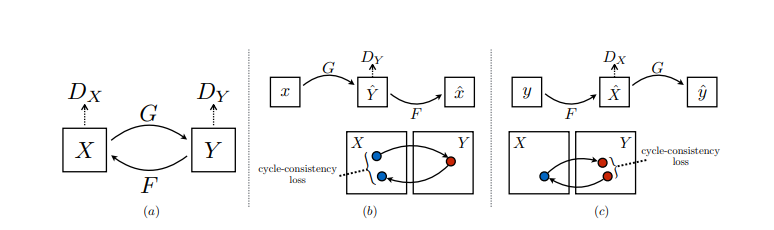
\includegraphics[scale=.57]{figuras/cycleconsistencyandlosses.png}
  \legend{Fonte: \cite{cycle-gan}}
  \label{fig:cycleconsistencyandlosses}
\end{figure}

A partir dos resultados dos experimentos realizados com o CycleGAN bem como a quantidade de dados disponíveis para alcançar tais resultados, optou-se por utilizar essa arquitetura e modelo como base para os testes do escopo em questão.

\subsubsection{Configuração do Modelo}

Como já é conhecido, um dos pontos principais que os modelos de GAN são negativamente referenciados é por conta do custo computacional e quantidade de dados exigidos para atingir resultados satisfatórios \cite{f8-decrappification}. Porém, a arquitetura do CycleGAN permite atingir resultados significativos com uma amostra de dados pequena \cite{cycle-gan}. No trabalho, os cientistas conseguiram fazer a transformação de imagens de cavalos (939 imagens) em zebras (1177 imagens) com pouco mais de 2000 (dois mil) imagens para treinamento e testes. Por isso, o processo de \textit{augmentation} visto na figura \ref{fig:data-augmentation} não será aplicado para o estudo do CycleGAN do presente trabalho.

A implementação do CycleGAN foi baseada em uma postagem publicada no Medium por Kayo Yin, com o título \href{https://medium.com/illuin/cleaning-up-dirty-scanned-documents-with-deep-learning-2e8e6de6cfa6}{\textit{Cleaning Up Dirty Scanned Documents with Deep Learning}}, construído a partir da biblioteca do Keras, em sua versão 2.0.8. O tamanho utilizado da imagem utilizado foi de 768x512x1.

Para a configuração dos modelos Gerador e Discriminador, utilizou-se os seguintes hiperparâmetros:

\begin{itemize}
  \item \textit{\textbf{batch\_size:}} o principal limitante para a definição desse hiperparâmetro foi a capacidade computacional disponível durante o desenvolvimento do trabalho. Para imagens do tamanho proposto, o único valor possível foi \textbf{1}, ou seja, o algoritmo consome uma imagem a cada iteração com a rede;
  \item \textbf{\textit{optimizer:}} utilizou-se o algoritmo de otimização Adam com \textit{learning rate} de 0.002;
  \item \textit{\textbf{loss\_function:}} para a função de erro, utilizou-se a MSE ou \textit{Mean Squared Error};
\end{itemize}

O sumário dos modelos Geradores são:

\begin{figure}[H]
  \centering
  \caption{Arquitetura das camadas dos modelos Geradores d CycleGAN.}
  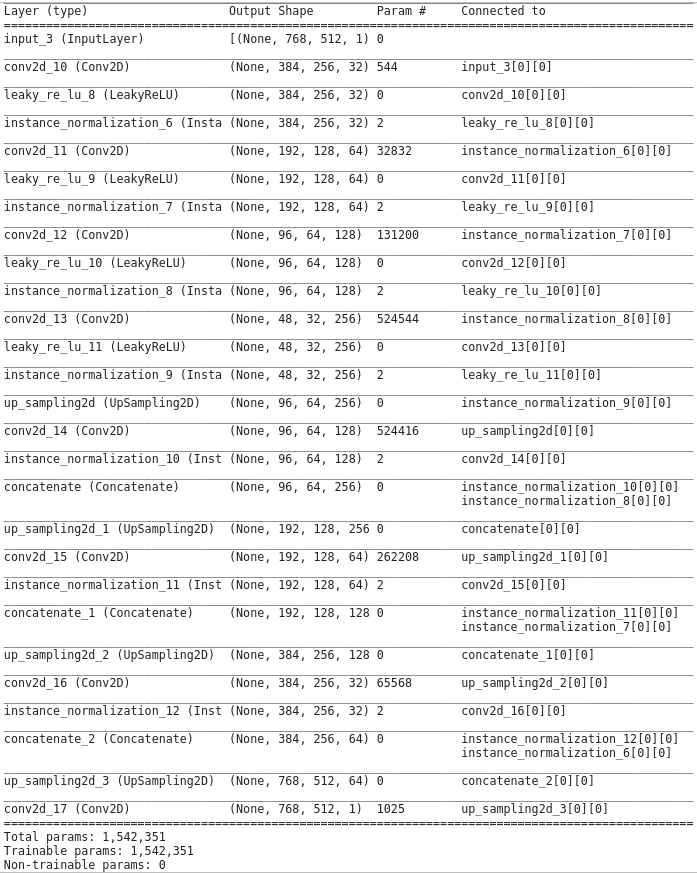
\includegraphics[scale=.55]{figuras/generator-architecture.png}
  \legend{Fonte: Autoral.}
  \label{fig:generator-architecture}
\end{figure}

\subsubsection{Resultados}

Inicialmente, utilizou-se o \textit{dataset} para treinamento, teste e validação em 70\%, 20\% e 10\%, respectivamente. Para tanto, como a quantidade de imagens é muito vasta, inicialmente testou-se o treinamento por cerca de 2 épocas. O tempo total para o treinamento foi de aproximadamente 19 horas, cerca de 9,5 horas por época. Pelo gráfico de evolução da \textit{loss} durante o processo de treinamento, tem-se:

\begin{figure}[H]
  \centering
  \caption{Gráfico de \textit{loss} do modelo Gerador da CycleGAN.}
  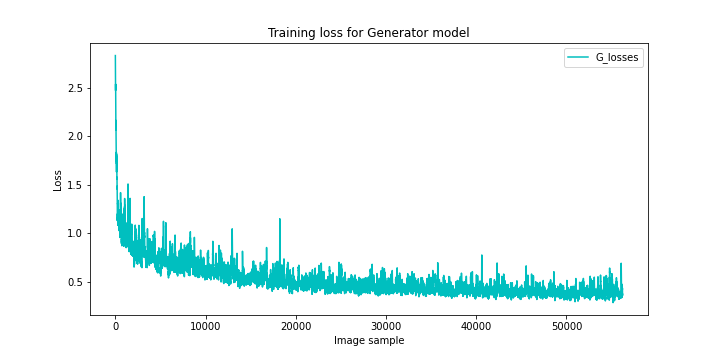
\includegraphics[scale=.55]{figuras/g_losses.png}
  \legend{Fonte: Autoral.}
  \label{fig:g_losses}
\end{figure}

Utilizando a MSE como métrica de \textit{loss}, é possível observar apenas pelo gráfico que a qualidade da imagem resultante do modelo Gerador é melhor do que a imagem \textit{crappy} de entrada, visto que é possível verificar que a perda tende a convergir \cite{everything-about-nn}.

Independente do modelo convergir, a métrica de \textit{loss} em questão não diz necessariamente que o modelo manteve as principais características da imagem, permitindo assim que o Tesseract desempenhe melhor a partir da métrica Rouge-N.

\begin{figure}[H]
  \centering
  \caption{CycleGAN com 2 épocas.}
  \begin{subfigure}[t]{.3\linewidth}
    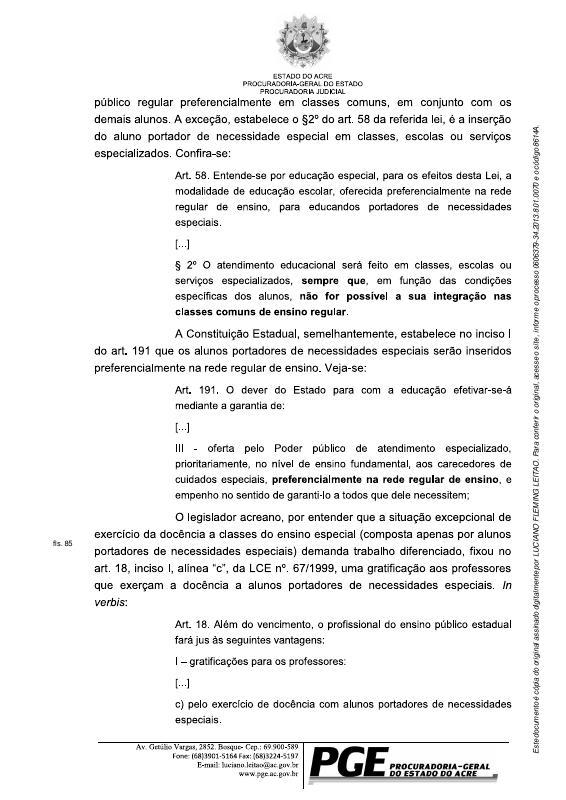
\includegraphics[width=\textwidth]{figuras/1004871_310554941_13.jpg}
    \caption{Original}
  \end{subfigure}
  \begin{subfigure}[t]{.3\linewidth}
    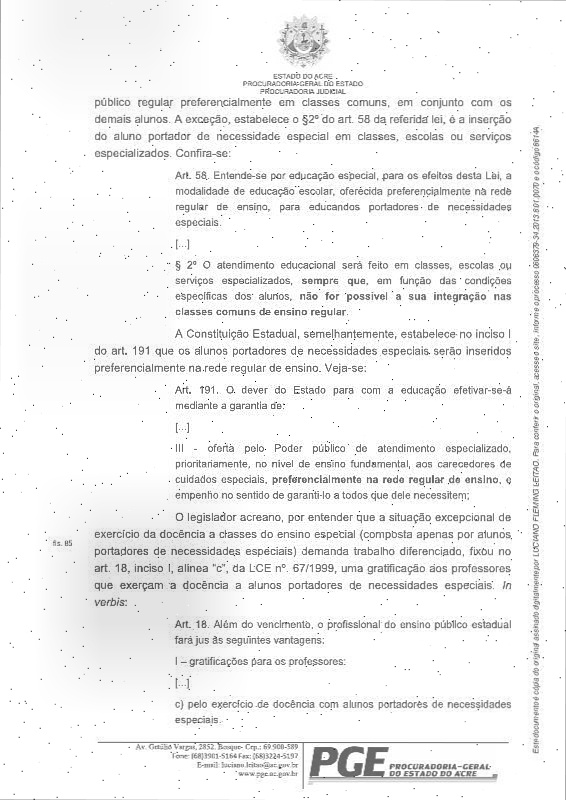
\includegraphics[width=\textwidth]{figuras/1004871_310554941_13_crappy.jpg}
    \caption{\textit{Crappy}}
  \end{subfigure}
  \begin{subfigure}[t]{0.3\linewidth}
    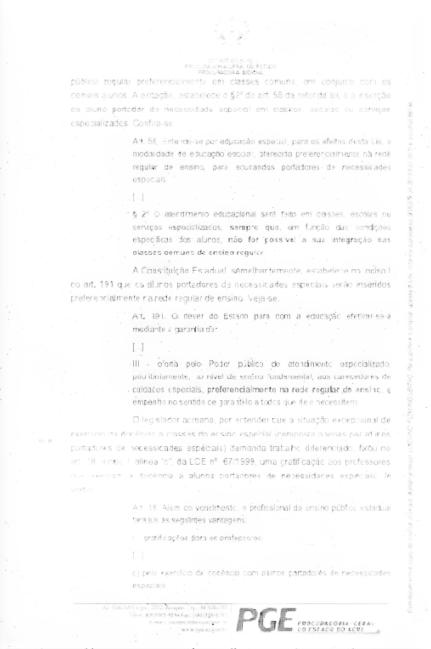
\includegraphics[width=\textwidth]{figuras/1004871_310554941_13_corrected.jpg}
    \caption{Corrigida}
  \end{subfigure}
  \legend{Fonte: autoral.}
  \label{fig:cycle-gan-first-test}
\end{figure}

% USAR O ARQUIVO ../crappy_images/1004871_310554941_13.jpg PARA TESTES
Nitidamente é possível observar que o conteúdo da imagem foi ofuscado pelo pré-processador. Extraindo a métrica Rouge das imagens acima, tem-se:

\begin{table}[H]
  \centering
  \caption{Resumo dos resultados iniciais do pré-processador CycleGAN em imagem de teste.}
  \begin{tabular}{|c|c|c|}
    \hline
      \textbf{Métrica}  &
      \textbf{Crappy}  &
      \textbf{Imagem corrigida} \\
    \hline
      Rouge-1  &
      0.734 &
      0.181 \\
    \hline
      Rouge-2  &
      0.544 &
      0.009 \\
    \hline
      Rouge-3  &
      0.432 &
      0.0 \\
    \hline
      Rouge-4  &
      0.318 &
      0.0 \\
    \hline
      Rouge-L &
      0.773 &
      0.231 \\
    \hline
  \end{tabular}
  \legend{Fonte: autoral}
  \label{tab:first-cycle-gan-rouge-n}
\end{table}

A partir da publicação do Medium que foi utilizada como base para a construção do algoritmo, bem como o desenvolvimento do mesmo processo por outra pessoa em \href{https://medium.com/towards-artificial-intelligence/cyclegan-as-a-denoising-engine-for-ocr-images-8d2a4988f769}{outra publicação}, observou-se que durante as épocas iniciais o modelo não foi capaz de manter o texto presente na imagem. Porém, com o avanço das épocas, a imagem resultante passou a conservar mais o sinal presente nela. Contudo, aumentar o número de épocas dentro do \textit{dataset} do projeto seria inviável, de acordo com o tempo médio de cada época sobre o dado completo. Com isso, iniciou-se os testes com um \textit{sample} de dados menor e mais controlado, permitindo assim que seja possível realizar o treinamento com mais épocas e verificar os resultados.

Para o resultado final do treinamento do algoritmo, separou-se randomicamente 5 mil imagens do \textit{dataset} completo e aumentou-se o número de épocas para X.

\textcolor{red}{VOLTAR AQUI E COLOCAR A TABELA RESULTANTE BEM COMO O NÚMERO FINAL DE ÉPOCAS}

\begin{table}[H]
  \centering
  \caption{Resumo dos resultados finais do pré-processador CycleGAN sobre o \textit{dataset} de testes.}
  \begin{tabular}{|c|c|c|}
    \hline
      \textbf{Métrica}  &
      \textbf{Crappy}  &
      \textbf{Imagem corrigida} \\
    \hline
      Rouge-1  &
      0.734 &
      0.181 \\
    \hline
      Rouge-2  &
      0.544 &
      0.009 \\
    \hline
      Rouge-3  &
      0.432 &
      0.0 \\
    \hline
      Rouge-4  &
      0.318 &
      0.0 \\
    \hline
      Rouge-L &
      0.773 &
      0.231 \\
    \hline
  \end{tabular}
  \legend{Fonte: autoral}
  \label{tab:cycle-gan-rouge-n-result}
\end{table}

\subsection{Pocessador \textit{Decrappification}}

O último passo para a o processo de desenvolvimento proposto foi a construção do pré-processador de imagem utilizando o método \textit{decrappification}. A principal motivação para a sua construção foi devido aos seus incríveis resultados como correção de imagens médicas bem como a utilização do mesmo para melhorar a qualidade de imagens de diferentes tipos \cite{f8-decrappification}.

Para a construção do algoritmo e testes com o modelo, utilizou-se a biblioteca do fast.ai em sua versão 1.1.6.

\subsubsection{Configuração do modelo}

Como comentado anteriormente na seção \ref{ssec:decrappification}, o modelo de \textit{decrappification} utiliza o \textit{transfer learning} sobre uma rede U-net \cite{u-net}. Tal rede pode ser criada a partir de algumas arquiteturas já existentes e a arquitetura utilizada para a construção do pré-processador foi a arquitetura Resnet34. Basicamente, quanto maior o número de camadas ou o quão mais profunda a rede é, mais difícil fica o seu treinamento \cite{deep-resnet-for-image-recognition}, por isso optou-se por utilizar uma rede sofisticada mas com um menor grau de camadas, para um treinamento mais rápido.

A implementação do \textit{deccrappification} foi baseada no curso do fast.ai \href{https://course.fast.ai/}\textit{Practical Deep Learning for Coders} na versão 1.

Para a configuração desse modelo durante o treinamento utilizou-se os seguintes parâmetros:

\begin{itemize}
  \item \textit{\textbf{batch\_size:}} novamente, o principal limitante para a definição desse hiperparâmetro foi a capacidade computacional. Aqui, utilizou-se imagens um pouco maiores, a ser explicado posteriormente e \textit{batch\_size} se manteve igual a \textbf{1};
  \item \textbf{\textit{optimizer:}} utilizou-se o algoritmo de otimização Adam com \textit{learning rate} padrão da biblioteca de 0.001;
  \item \textit{\textbf{loss\_function:}} MSE ou \textit{Mean Squared Error};
\end{itemize}

A arquitetura Resnet bem como a U-net foram construíadas com foco em imagens quadradas, como 256x256 para a U-net \cite{u-net}, mas como comentado anteriormente, o \textit{dataset} contém imagens retangulares. O próprio fast.ai implementa alguns transformadores do dado de treinamento e teste mas ele realiza um corte na imagem a partir do tamanho configurado e não adapta de fato a imagem original. Portanto, foi necessário realizar a adaptação das imagens retangulares dos documentos para um tamanho quadrado. O tamanho a ser testado foi de 768x768, com a mesma altura utilizada nos modelos anteriores de CycleGAN.

Em média, as imagens presentes no \textit{dataset} são imagens com o tamanho próximo a 800x512. Em testes de alteração da imagem frente ao impacto do mesmo no resultado do Tesseract, observou-se que ao realizar a adaptação de acordo com a altura (\textit{height}) da imagem, a métrica Rouge-L obteve média de 0.621 frente a 0.277 quando adaptado-se em relação a largura (\textit{width}) da mesma. O teste foi realizado em uma amostra de 100 imagens do \textit{dataset} original.

Tal modelo acaba trazendo uma complexidade maior para o pré-processador a ser construído, visto que após o \textit{predict} do modelo sobre uma imagem \textit{crappy} para a possível correção, será necessário realizar a adaptação da imagem para o seu tamanho original para então utiliza-la como entrada para o algoritmo do Tesseract.


\subsubsection{Resultados}

Para o processo de construção do pré-processador em questão, utilizou-se para treinamento, teste e validação em 70\%, 20\% e 10\%, respectivamente. Mesmo para imagens maiores utilizadas no \textit{decrappification}, o algoritmo obteve médias próximas a 6 horas e 40 minutos por época. Utilizou-se 2 épocas para o treinamento.

Por se tratar de um modelo que utiliza \textit{transfer learning}, espera-se que o processo de aprendizagem seja mais eficiente do que treinando-se uma rede inteiramente do início, sem inicialização de pesos adequada, como vista no CycleGAN, e que com isso a \textit{loss function} tenda a convergir mais rapidamente. Isso é possível verificar no gráfico de \textit{loss} do modelo \textit{decrappification}.

\textcolor{red}{VOLTAR AQUI E COLOCAR A LOSS DO DECRAP}
